%-----------------------------------------------------------------------
\chapter{Conclusions and Future Work}
\section{Conclusions}
The objective of our project was to produce a prototype pipeline that takes captured facial performance as input, and creates an animation of a three-dimensional model of a human face. 

The quality of an animation may be evaluated in a number of different ways. In our final animated sequence Emily is able to closely mimic the motion of the actor while retaining individuality imposed by the structure and features of Emily's face. The realism of our animations improved with time; the first animation has no eyes or mouth, and it exhibits unusual behaviours. On the contrary, the final animation includes motion of the eyes and the teeth, as well as more plausible overall performance, thus it looks significantly more appealing. Though more realistic than a hand-drawn character or an industrial robot, our results lack the naturalness of human motion. We believe that our results belong in the uncanny valley of the familiarity versus human likeness diagram, see Fig.~\ref{fig:UV}. The theory of the uncanny valley suggests that human-like appearance and behaviour is perceived as repulsive as the resemblance increases~\cite{UV}.
\begin{figure}[htbp!]
\centering
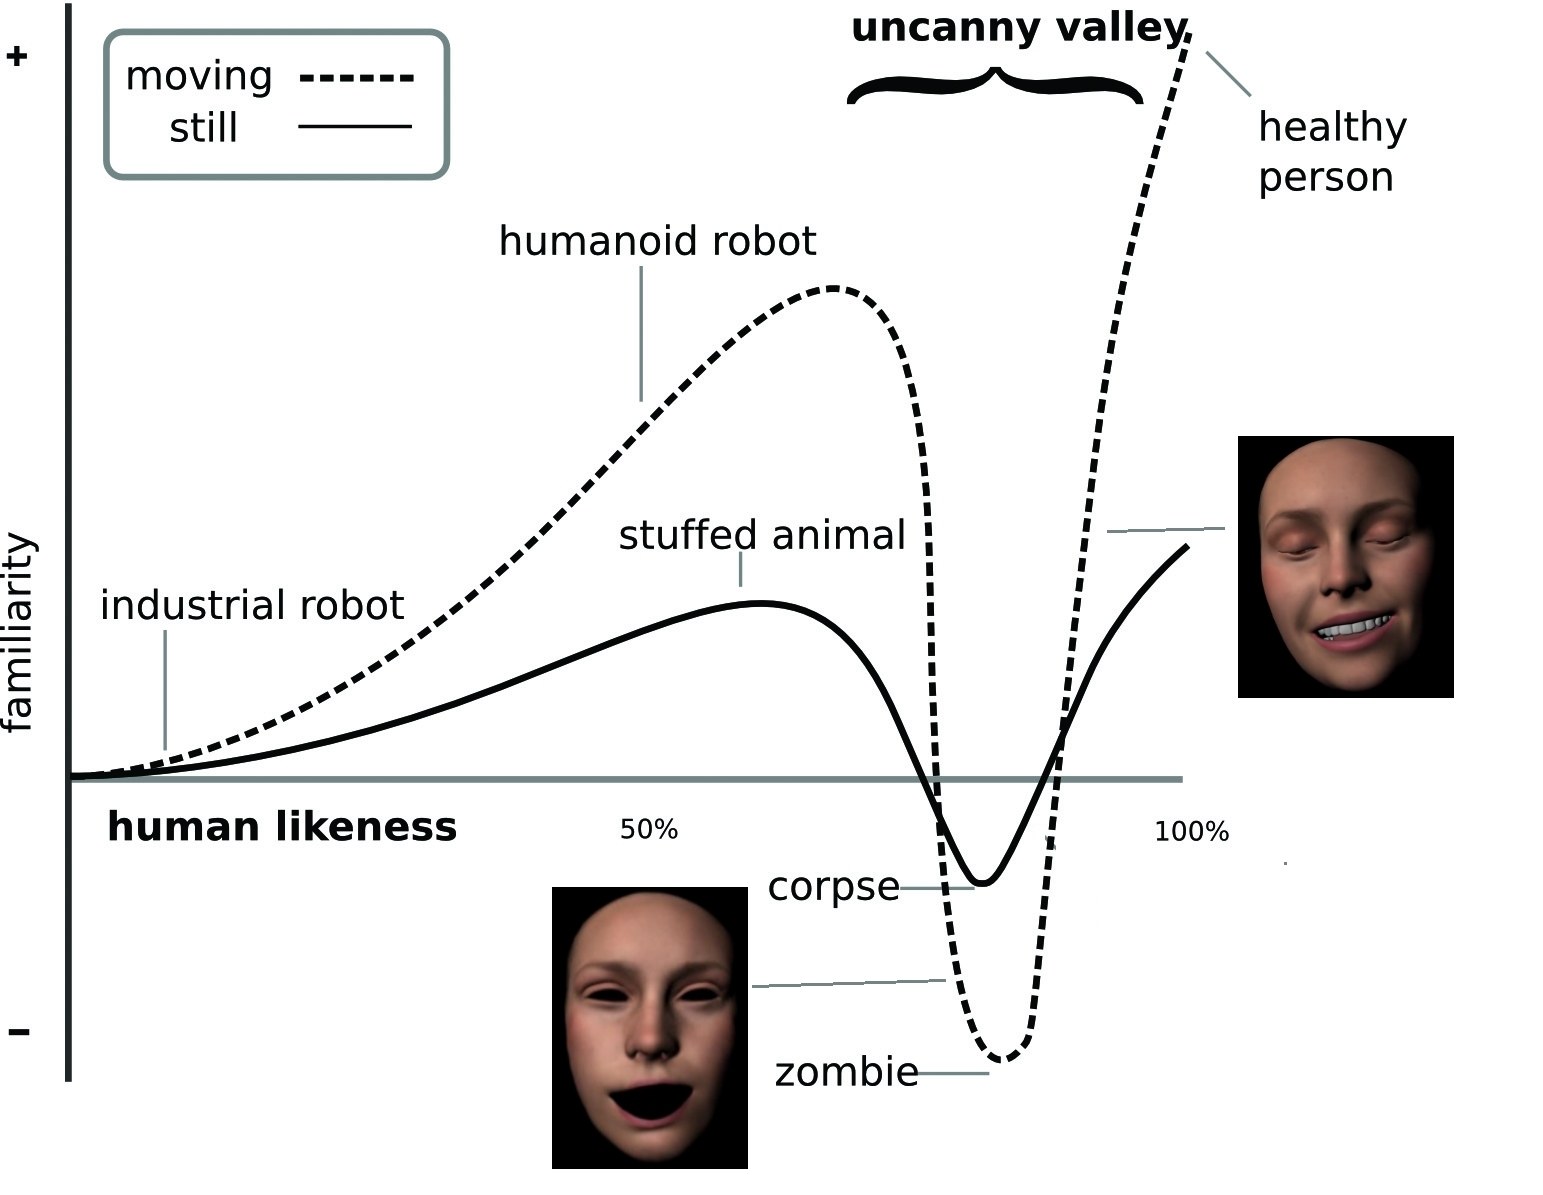
\includegraphics[width=0.8\textwidth]{img/UV}
	\caption{Our animations in the context of the uncanny valley.}
	\label{fig:UV}
\end{figure}

% Rendering was improved when doing super-resolution on the textures.
% Improvement only noticeable at close ups
% Improvement was only marginal


\section{Future Work}

There are a number of different techniques that could be used to construct blendshapes in the actor's domain. Deng et al. proposed designing the blendshapes by hand~\cite{Deng:2006}. In particular, the authors choose a number of characteristic frames in the motion capture sequence, and manually design a set of shapes that perceptually match the expressions observed in these frames. They then form correspondences between the PCA coefficients of motion capture frames and the weights of the blendshapes. Finally, Radial Basis Functions are used to map the new frames in the sequence onto the three-dimensional model to produce the animation. Another option would be to use a muscle actuation basis, proposed by Choe and Ko~\cite{Choe:2005}. The design of a muscle actuation basis is based on the human facial anatomy, and is driven by the actuation of different facial muscles. Our main reservation about these approach is the extensive manual effort required to design the set of initial correspondences between the chosen frames and the three-dimensional mesh.

The accuracy of the model may be improved by taking extra care when matching the sparse points on Emily and the actor. One possible approach involves drawing a number of stable points on Emily and the actor and finding the mapping that transforms sparse Emily points to the actor's domain. Then a large number of additional points are drawn on Emily, and the same transformation is used to transform these points to the actor's domain. These points are then used to identify the ideal location of the markers on the actor's face. Moreover, a 3D printed mask may be used to ensure high accuracy when placing the markers. % THIS PARAGRAPH DOESN'T SOUND RIGHT. I FORGOT WHAT I WAS TRYING TO DAY.

The main weakness of the current method is the amount of manual work that needs to be done before the animation takes its final shape. 
% We could track eyelids and add blinks automatically.


The realism of the final animation could also be enhanced by applying more complex skin rendering techniques.
In this line, we could add layered materials which model subsurface scattering in the skin \cite{Weyrich2006}.
A further extension would be to include haemoglobin related phenomena, as proposed by~\cite{Donner2008, Jimenez2010}.
Adding bump maps or normals maps also increases the quality of the final result, however a light stage  is needed to acquire such data with enough resolution~\cite{Graham2013}.

% Including wrinkles.

% Talk about adding BSSRDF to the skin rendering
% Adding normal maps for more detail -> capture studio with light dome